\chapter{Previous work}
\label{ch:previous_work}

As stated in the problem statement in section \ref{sec:problem} the focus of the implementations underlying this thesis is to implement multiple strategies to extract a triangulated surface mesh from the data model used inside the VML.
To aid the reader in understanding the implementations present in this thesis, a short introduction to the VML and its data model is given.
Parts of this description have been taken from the authors bachelor thesis where the data model has been previously described with the focus on visualization \cite{bachelor}.

\section{Project history}
\label{sec:project_history}

From mid 2011 until the end of 2013 project Enlight was conducted for research by the RISC Software GmbH in Hagenberg im M\"uhlkreis, Austria.
Enlight's goals were to develop a faster, scalable and numerically stable method for modeling and visualizing subtractive manufacturing.
Enlight used a regular grid data structure to store a stock solid and add precomputed swept volumes.
A triangle elimination strategy was employed to keep the total number of triangles held by the grid within manageable bounds.
For visualization a customized ray casting approach was developed \cite{enlight} and accelerated using GPUs and many-core architectures.

From the beginning to the end of 2014, the follow-up research project Engrave focused on solving swept volume computation for arbitrary cutter geometries and tool paths.
Engrave basically allowed dynamic swept volume computation from a set of cutter solids and transformation lists.
Swept volume computation was done by extruding a point cloud along the tool path and then reconstruction a closed triangle mesh from it using a parallel and highly optimized variant of the ball pivoting algorithm 
\cite{engrave}.
The computed swept volumes where directly imported into Enlight's data model.

Both projects, Enlight and Engrave, were co-funded by the European Union as well as Land Ober\"osterreich within the political program Regio 13, which aimed to sustainably improve the contestability of regional companies, economic growth and employment inside of Upper Austria.
%
With the beginning of 2015 the prototype developed during Enlight and Engrave was rebranded to Virtual Machining Library (VML) and is currently further developed as a commercial product.

\section{VML data model}
\label{sec:vml_data_model}

The primary purpose of the VML is to model, simulate and visualize subtractive manufacturing.
A typical workflow consists of loading a stock solid and then repeatedly sweeping various cutting tools over the stock.
These cutting tools are solid triangle meshes loaded from disk which are moved along paths (list of transformation matrices) to create swept volumes (generated triangle meshes).
These swept volumes are then conceptually subtracted from the stock.
In fact, swept volumes are stored side by side together with the stock and theoretically build up a specialized CSG tree as shown in figure \ref{fig:vml_csg}.
A separate processing step is required to calculate the exact surface.
For visualization, the data model is sampled using a raycast which calculates a point on the surface for each ray.

\begin{figure}
	\centering
	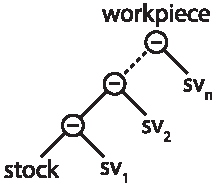
\includegraphics[width=0.5\textwidth]{images/vml_csg}
	\caption{
		The input model held by the VML can be seen as a linearized CSG tree.
		The initial stock solid is combined with a series of swept volumes using boolean subtraction.
		The VML stores parts of the geometries of all leaves of this tree (\cf classification \ref{sec:classification}).
	}
	\label{fig:vml_csg}
\end{figure}


The central data structure inside the VML which holds the current state of the simulation (\ie the workpiece) is a regular 3-dimensional grid.
This data structure was chosen because, historically, it was directly used as acceleration structure for the raycasting subsystem.
Although there is a wide variety of acceleration structures available (\eg kd-trees, octrees, binary space partitioning (BSP), bounding volume hierarchies (BVH), \etc), regular grid offer greater simplicity in organization and construction than the others.
This is especially beneficial in cases where those data structures have to be updated regularly.
Particularly animated scenes in computer-animated films or changing geometries as in virtual machining require frequent rebuilds or updates of those data structures.
Due to their simplicity and regularity, regular grids provide viable candidates for these scenarios.
However, the VML's regular grid is also the basis for a triangle count optimization called classification which is described in the following section.


\subsection{Classification}
\label{sec:classification}

Every time a solid triangle mesh (stock or swept volume) is added to the grid, the triangles of the mesh have to be mapped to the cells of the grid.
Thereby, each triangle is added to each cell it intersects.
A triangle is therefore potentially referenced from multiple cells.
When the mapping is complete, the affected cells are classified into one of three categories with respect to the newly added mesh.
Cells which are occupied by triangles of the mesh's surface are surface cells.
Cells inside and outside the mesh are inside and outside cells and contain no triangles.
The sketch in Figure \ref{fig:classification_before} illustrates the classification of a single solid inside the grid (\ie stock).

\begin{figure}[h]
	\centering
	\begin{subfigure}[b]{0.4\textwidth}
		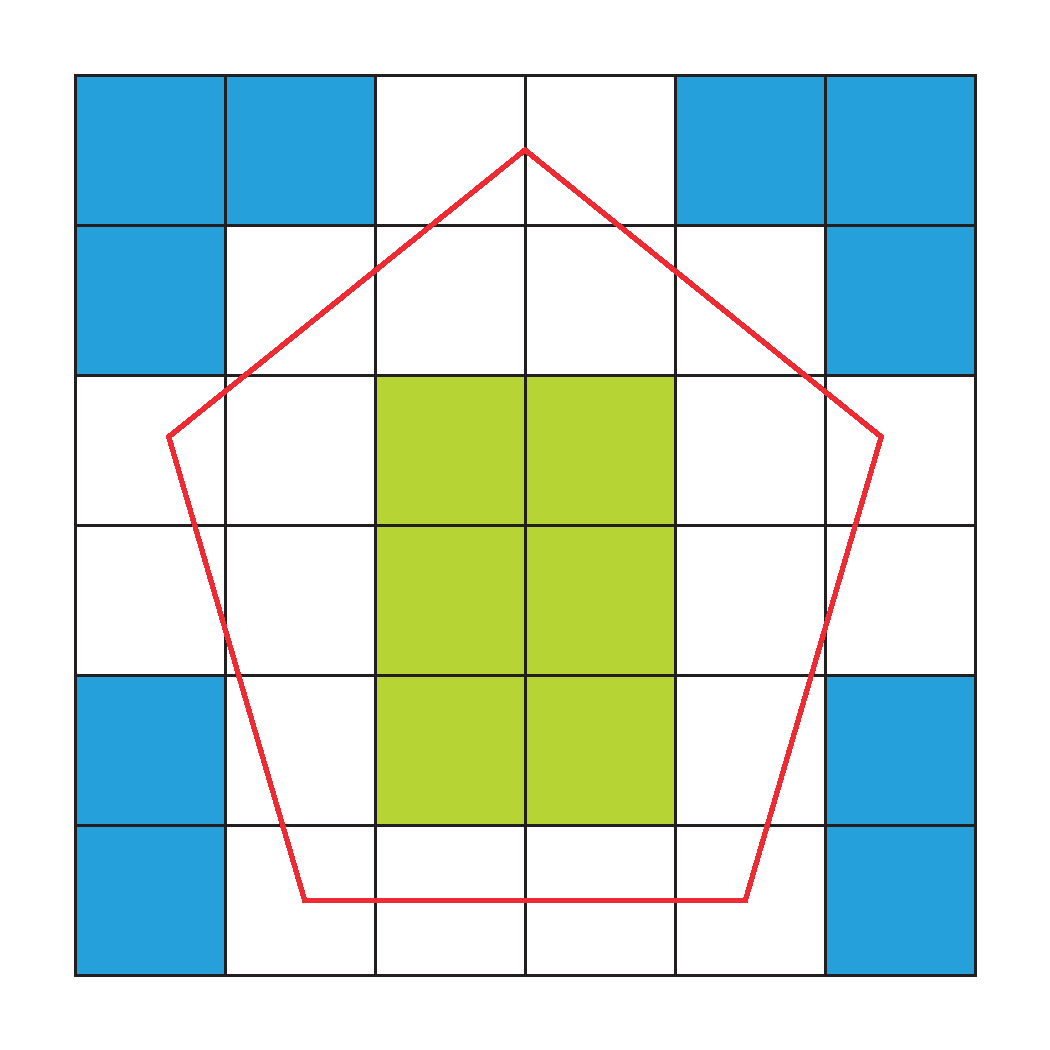
\includegraphics[width=\textwidth]{images/classification_before}
		\caption{Classification of the regular grid after a stock volume has been added.}
		\label{fig:classification_before}
	\end{subfigure}
	\begin{subfigure}[b]{0.4\textwidth}
		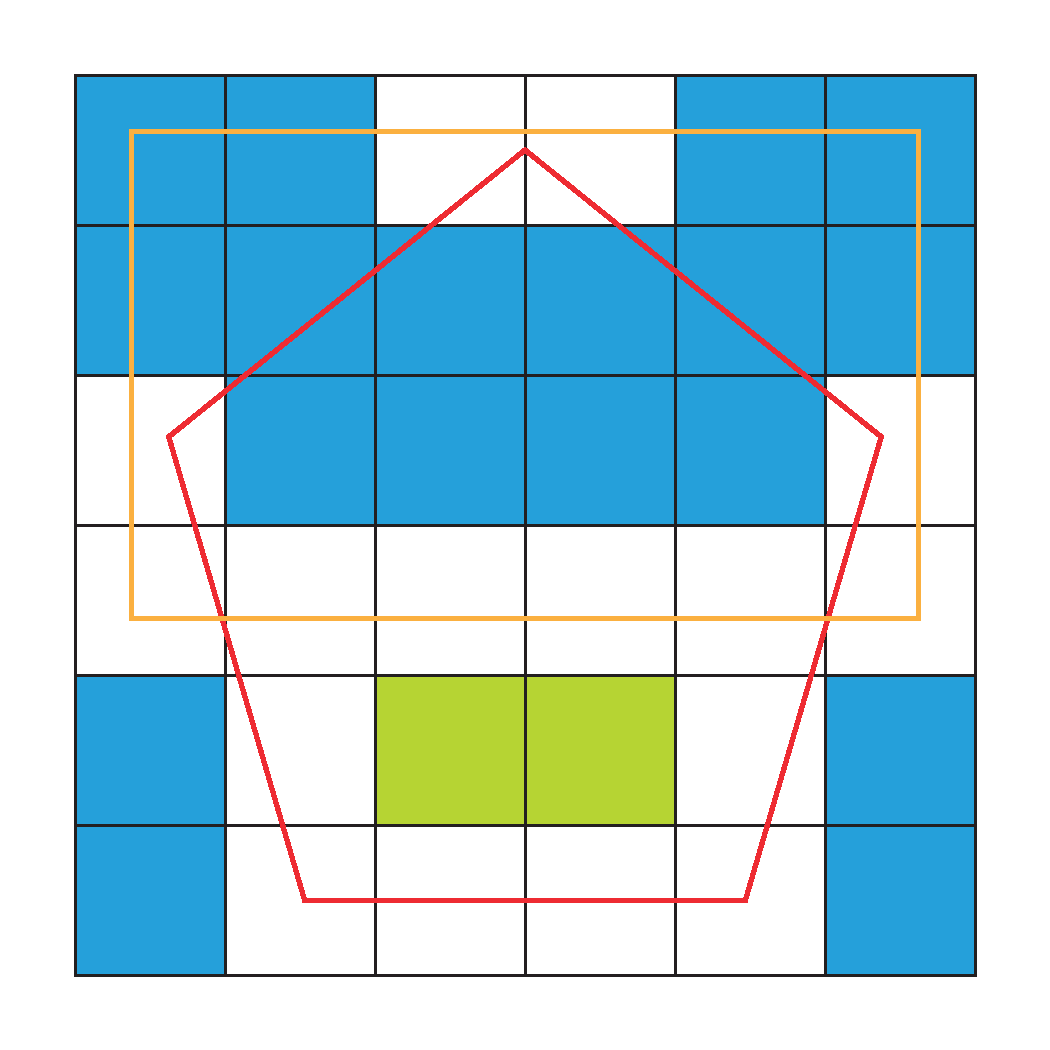
\includegraphics[width=\textwidth]{images/classification_after}
		\caption{Classification of the regular grid after a swept volume has been added to the stock.}
		\label{fig:classification_after}
	\end{subfigure}
	\caption{Principle of classifying cells of a grid according to the added mesh. Only surface cells are relevant for ray casting. The sketch on the left side shows the classified stock solid. On the right side the classification result after adding a swept volume is shown.}
	\label{fig:classification}
\end{figure}

When a new mesh is added to the grid, the mesh is again classified and merged into the existing cell classification. Limiting the modifiability of the scene by only allowing the addition of subtraction volumes simplifies the rules for merging a new mesh into the grid as shown in Table \ref{tbl:classification_rules}.

\begin{table}[h]
	\centering
	\begin{tabular}{|c|c|c|c|c|}
		\hline
		\multicolumn{2}{|c|}{\multirow{2}{*}{merge}} & \multicolumn{3}{c|}{Cell class of subtraction volume} \\
		\cline{3-5}
		\multicolumn{2}{|c|}{} & outside & surface & inside \\
		\hline
		\multirow{3}{*}{Cell class before} & outside & outside & outside & outside \\
		\cline{2-5}
		& surface & surface & surface & outside \\
		\cline{2-5}
		& inside & inside & surface & outside \\
		\hline
	\end{tabular}
	\caption{Table of different merge scenarios and their outcome.}
	\label{tbl:classification_rules}
\end{table}

Cells which are outside the added subtraction volume remain unchanged. Surface cells of the added volume become surface cells except they where outside cells before, and cells inside a subtraction volume always become outside cells, as they lie outside the resulting geometry. The result of merging a subtraction volume into the grid is visualized in the right sketch in Figure \ref{fig:classification}.

As we can see, cells which where surface cells before and contained triangles have now changed to outside cells and are therefore no longer relevant for ray casting. As a result, the increase of triangles in the surface cells by adding new volumes has been compensated by exclusion of some surface cells. This reduction of potential triangles for intersection with an increasing number of subtraction volumes is vital, as it enables scalability, allowing even scenes with thousands of subtraction volumes to be ray casted efficiently. In fact, some scenes can even be casted faster with an increasing number of subtraction volumes as the number of relevant surface cells and therefore triangles decreases.

However, this kind of reduction has a significant consequence on the ray casting algorithm. As subtraction volumes are divided into grid cells and some of them discarded, the volumes are no longer water-tight. This is a problem for entry/exit counting ray casting algorithms such as the one discussed in chapter \ref{sec:boolean_raycasting}. Therefore, an adapted version of this algorithm has to be developed, capable of handling open volumes. Chapter \ref{sec:adapted_ray_casting} discusses a method of getting around this problem.

\subsection{Visualization by raycasting}
\label{sec:raycasting}

cell traversal using 3D DDA
inside counting (secondary rays, etc.)
determining surface

optimization by packet casting


%TODO


A vital requirement of such systems is to support a large number of fine triangulated meshes (up to hundreds of millions of triangles) to deliver simulations of appropriate quality.
Therefore, well-conceived space partitioning and triangle elimination strategies have been developed to deal with this amount of input.

As a result the simulated model is described implicitly via subtraction of only subsets of the input triangles (volumes are no longer closed/water-tight).

For visualization, this implicit model is sampled using an adapted ray casting approach \cite{enlight}.
By applying a small set of rules, the surface can be recovered to retrieve an image of the model.
Enlight's data model is described in detail in the author's bachelor thesis \cite{bachelor}.

Simulation and visualization of material removal processes such as in Enlight are vital for verifying the correctness of a machining process.
However, there exist numerous scenarios where an explicit surface model of the final product is required.
Many of these situations occur in CAE such as stress, thermal and safety analyses as well as structural optimizations using finite element methods.
Due to the importance for CAE for assuring quality in modern production processes it is highly desired to be able to retrieve an explicit surface mesh of the implicitly described model of Enlight.

